
\documentclass[xcolor=dvipsnames]{beamer}  % for hardcopy add 'trans'

\mode<presentation>
{
  \usetheme{Singapore}
  % or ...
  \setbeamercovered{transparent}
  % or whatever (possibly just delete it)
}

\usefonttheme{professionalfonts}
%\usepackage[english]{babel}
% or whatever
%\usepackage[latin1]{inputenc}
% or whatever
%\usepackage{times}
%\usepackage[T1]{fontenc}
% Or whatever. Note that the encoding and the font should match. If T1
% does not look nice, try deleting the line with the fontenc.

%%%%%%%%%%%%%%%%%%%%%% start my preamble %%%%%%%%%%%%%%%%%%%%%%


\addtobeamertemplate{navigation symbols}{}{%
    \usebeamerfont{footline}%
    \usebeamercolor[fg]{footline}%
    \hspace{1em}%
    \insertframenumber/\inserttotalframenumber
}

\setbeamercolor{footline}{fg=blue}
\setbeamerfont{footline}{series=\bfseries}


%\usepackage{epsfig}
\usepackage{graphicx}
\usepackage{amsmath, amssymb, amsthm}

\usepackage{fancyvrb}

\usepackage{tikz}
\usetikzlibrary{arrows}
\usetikzlibrary{calc}
\usetikzlibrary{intersections}
\usetikzlibrary{decorations}
\usepackage{pgf}
\usepackage{pgfplots}
\pgfplotsset{compat=1.13}

\usepackage{graphviz}
 
\usepackage{verbatim}


\usepackage{algorithmicx,algpseudocode}


%font
\usepackage{mathpazo}
%\usepackage[usenames, dvipsnames]{color}

%\usepackage[linesnumbered, ruled, lined]{algorithm2e}

\usepackage{xr}
\externaldocument[ET-]{et}


\newcommand*{\theorembreak}{\usebeamertemplate{theorem end}\framebreak\usebeamertemplate{theorem begin}}

\newcommand{\newtopic}[1]{\textcolor{Green}{\Large \bf #1}}
\newcommand{\navy}[1]{\textcolor{Blue}{\bf #1}}
\newcommand{\navymth}[1]{\textcolor{Blue}{#1}}
\newcommand{\red}[1]{\textcolor{red}{#1}}


\definecolor{pale}{RGB}{235, 235, 235}
\definecolor{pale2}{RGB}{175,238,238}
\definecolor{turquois4}{RGB}{0,134,139}

% Typesetting code
\definecolor{bg}{rgb}{0.95,0.95,0.95}
\usepackage{minted}
\usemintedstyle{friendly}
\newminted{python}{mathescape,frame=lines,framesep=4mm,bgcolor=bg}
\newminted{ipython}{mathescape,frame=lines,framesep=4mm,bgcolor=bg}
\newminted{julia}{mathescape,frame=lines,framesep=4mm,bgcolor=bg}
\newminted{c}{mathescape,linenos=true}
\newminted{r}{mathescape,  frame=none, baselinestretch=1, framesep=2mm}
\renewcommand{\theFancyVerbLine}{\sffamily
    \textcolor[rgb]{0.5,0.5,1.0}{\scriptsize {\arabic{FancyVerbLine}}}}


\usepackage{stmaryrd}

\newcommand{\Fact}{\textcolor{Brown}{\bf Fact. }}
\newcommand{\Facts}{\textcolor{Brown}{\bf Facts }}
\newcommand{\keya}{\textcolor{turquois4}{\bf Key Idea. }}
\newcommand{\Factnodot}{\textcolor{Brown}{\bf Fact }}
\newcommand{\Eg}{\textcolor{ForestGreen}{Example. }}
\newcommand{\Egs}{\textcolor{ForestGreen}{Examples. }}
\newcommand{\Ex}{{\bf Ex. }}
\newcommand{\Thm}{\textcolor{Brown}{\bf Theorem. }}
\newcommand{\Prf}{\textcolor{turquois4}{\bf Proof.}}
\newcommand{\Ass}{\textcolor{turquois4}{\bf Assumption.}} 
\newcommand{\Lem}{\textcolor{Brown}{\bf Lemma. }}

%source code 



% caligraphic
\usepackage{mathrsfs}
\usepackage{bbm}
\usepackage{subfigure}

\newcommand{\argmax}{\operatornamewithlimits{argmax}}
\newcommand{\argmin}{\operatornamewithlimits{argmin}}

\newcommand\T{{\mathpalette\raiseT\intercal}}
\newcommand\raiseT[2]{\raisebox{0.25ex}{$#1#2$}}

\DeclareMathOperator{\cl}{cl}
%\DeclareMathOperator{\argmax}{argmax}
\DeclareMathOperator{\interior}{int}
\DeclareMathOperator{\Prob}{Prob}
\DeclareMathOperator{\kernel}{ker}
\DeclareMathOperator{\diag}{diag}
\DeclareMathOperator{\sgn}{sgn}
\DeclareMathOperator{\determinant}{det}
\DeclareMathOperator{\trace}{trace}
\DeclareMathOperator{\Span}{span}
\DeclareMathOperator{\rank}{rank}
\DeclareMathOperator{\cov}{cov}
\DeclareMathOperator{\corr}{corr}
\DeclareMathOperator{\range}{rng}
\DeclareMathOperator{\var}{var}
\DeclareMathOperator{\mse}{mse}
\DeclareMathOperator{\se}{se}
\DeclareMathOperator{\row}{row}
\DeclareMathOperator{\col}{col}
\DeclareMathOperator{\dimension}{dim}
\DeclareMathOperator{\fracpart}{frac}
\DeclareMathOperator{\proj}{proj}
\DeclareMathOperator{\colspace}{colspace}

\providecommand{\inner}[1]{\left\langle{#1}\right\rangle}

% mics short cuts and symbols
% mics short cuts and symbols
\newcommand{\st}{\ensuremath{\ \mathrm{s.t.}\ }}
\newcommand{\setntn}[2]{ \{ #1 : #2 \} }
\newcommand{\cf}[1]{ \lstinline|#1| }
\newcommand{\otms}[1]{ \leftidx{^\circ}{#1}}

\newcommand{\fore}{\therefore \quad}
\newcommand{\tod}{\stackrel { d } {\to} }
\newcommand{\tow}{\stackrel { w } {\to} }
\newcommand{\toprob}{\stackrel { p } {\to} }
\newcommand{\toms}{\stackrel { ms } {\to} }
\newcommand{\eqdist}{\stackrel {\textrm{ \scriptsize{d} }} {=} }
\newcommand{\iidsim}{\stackrel {\textrm{ {\sc iid }}} {\sim} }
\newcommand{\1}{\mathbbm 1}
\newcommand{\dee}{\,{\rm d}}
\newcommand{\given}{\, | \,}
\newcommand{\la}{\langle}
\newcommand{\ra}{\rangle}

\renewcommand{\rho}{\varrho}

\newcommand{\htau}{ \hat \tau }
\newcommand{\hgamma}{ \hat \gamma }

\newcommand{\boldx}{ {\mathbf x} }
\newcommand{\boldu}{ {\mathbf u} }
\newcommand{\boldv}{ {\mathbf v} }
\newcommand{\boldw}{ {\mathbf w} }
\newcommand{\boldy}{ {\mathbf y} }
\newcommand{\boldb}{ {\mathbf b} }
\newcommand{\bolda}{ {\mathbf a} }
\newcommand{\boldc}{ {\mathbf c} }
\newcommand{\boldi}{ {\mathbf i} }
\newcommand{\bolde}{ {\mathbf e} }
\newcommand{\boldp}{ {\mathbf p} }
\newcommand{\boldq}{ {\mathbf q} }
\newcommand{\bolds}{ {\mathbf s} }
\newcommand{\boldt}{ {\mathbf t} }
\newcommand{\boldz}{ {\mathbf z} }

\newcommand{\boldzero}{ {\mathbf 0} }
\newcommand{\boldone}{ {\mathbf 1} }

\newcommand{\boldalpha}{ {\boldsymbol \alpha} }
\newcommand{\boldbeta}{ {\boldsymbol \beta} }
\newcommand{\boldgamma}{ {\boldsymbol \gamma} }
\newcommand{\boldtheta}{ {\boldsymbol \theta} }
\newcommand{\boldxi}{ {\boldsymbol \xi} }
\newcommand{\boldtau}{ {\boldsymbol \tau} }
\newcommand{\boldepsilon}{ {\boldsymbol \epsilon} }
\newcommand{\boldmu}{ {\boldsymbol \mu} }
\newcommand{\boldSigma}{ {\boldsymbol \Sigma} }
\newcommand{\boldOmega}{ {\boldsymbol \Omega} }
\newcommand{\boldPhi}{ {\boldsymbol \Phi} }
\newcommand{\boldLambda}{ {\boldsymbol \Lambda} }
\newcommand{\boldphi}{ {\boldsymbol \phi} }

\newcommand{\Sigmax}{ {\boldsymbol \Sigma_{\boldx}}}
\newcommand{\Sigmau}{ {\boldsymbol \Sigma_{\boldu}}}
\newcommand{\Sigmaxinv}{ {\boldsymbol \Sigma_{\boldx}^{-1}}}
\newcommand{\Sigmav}{ {\boldsymbol \Sigma_{\boldv \boldv}}}

\newcommand{\hboldx}{ \hat {\mathbf x} }
\newcommand{\hboldy}{ \hat {\mathbf y} }
\newcommand{\hboldb}{ \hat {\mathbf b} }
\newcommand{\hboldu}{ \hat {\mathbf u} }
\newcommand{\hboldtheta}{ \hat {\boldsymbol \theta} }
\newcommand{\hboldtau}{ \hat {\boldsymbol \tau} }
\newcommand{\hboldmu}{ \hat {\boldsymbol \mu} }
\newcommand{\hboldbeta}{ \hat {\boldsymbol \beta} }
\newcommand{\hboldgamma}{ \hat {\boldsymbol \gamma} }
\newcommand{\hboldSigma}{ \hat {\boldsymbol \Sigma} }

\newcommand{\boldA}{\mathbf A}
\newcommand{\boldB}{\mathbf B}
\newcommand{\boldC}{\mathbf C}
\newcommand{\boldD}{\mathbf D}
\newcommand{\boldI}{\mathbf I}
\newcommand{\boldL}{\mathbf L}
\newcommand{\boldM}{\mathbf M}
\newcommand{\boldP}{\mathbf P}
\newcommand{\boldQ}{\mathbf Q}
\newcommand{\boldR}{\mathbf R}
\newcommand{\boldX}{\mathbf X}
\newcommand{\boldU}{\mathbf U}
\newcommand{\boldV}{\mathbf V}
\newcommand{\boldW}{\mathbf W}
\newcommand{\boldY}{\mathbf Y}
\newcommand{\boldZ}{\mathbf Z}

\newcommand{\bSigmaX}{ {\boldsymbol \Sigma_{\hboldbeta}} }
\newcommand{\hbSigmaX}{ \mathbf{\hat \Sigma_{\hboldbeta}} }

\newcommand{\RR}{\mathbbm R}
\newcommand{\CC}{\mathbbm C}
\newcommand{\NN}{\mathbbm N}
\newcommand{\PP}{\mathbbm P}
\newcommand{\EE}{\mathbbm E \nobreak\hspace{.1em}}
\newcommand{\EEP}{\mathbbm E_P \nobreak\hspace{.1em}}
\newcommand{\ZZ}{\mathbbm Z}
\newcommand{\QQ}{\mathbbm Q}


\newcommand{\XX}{\mathcal X}

\newcommand{\aA}{\mathcal A}
\newcommand{\fF}{\mathscr F}
\newcommand{\bB}{\mathscr B}
\newcommand{\iI}{\mathscr I}
\newcommand{\rR}{\mathscr R}
\newcommand{\dD}{\mathcal D}
\newcommand{\lL}{\mathcal L}
\newcommand{\llL}{\mathcal{H}_{\ell}}
\newcommand{\gG}{\mathcal G}
\newcommand{\hH}{\mathcal H}
\newcommand{\nN}{\textrm{\sc n}}
\newcommand{\lN}{\textrm{\sc ln}}
\newcommand{\pP}{\mathscr P}
\newcommand{\qQ}{\mathscr Q}
\newcommand{\xX}{\mathcal X}

\newcommand{\ddD}{\mathscr D}


\newcommand{\R}{{\texttt R}}
\newcommand{\risk}{\mathcal R}
\newcommand{\Remp}{R_{{\rm emp}}}

\newcommand*\diff{\mathop{}\!\mathrm{d}}
\newcommand{\ess}{ \textrm{{\sc ess}} }
\newcommand{\tss}{ \textrm{{\sc tss}} }
\newcommand{\rss}{ \textrm{{\sc rss}} }
\newcommand{\rssr}{ \textrm{{\sc rssr}} }
\newcommand{\ussr}{ \textrm{{\sc ussr}} }
\newcommand{\zdata}{\mathbf{z}_{\mathcal D}}
\newcommand{\Pdata}{P_{\mathcal D}}
\newcommand{\Pdatatheta}{P^{\mathcal D}_{\theta}}
\newcommand{\Zdata}{Z_{\mathcal D}}




\newcommand{\e}[1]{\mathbbm{E}[{#1}]}
\newcommand{\p}[1]{\mathbbm{P}({#1})}

%\theoremstyle{plain}
%\newtheorem{axiom}{Axiom}[section]
%\newtheorem{theorem}{Theorem}[section]
%\newtheorem{corollary}{Corollary}[section]
%\newtheorem{lemma}{Lemma}[section]
%\newtheorem{proposition}{Proposition}[section]
%
%\theoremstyle{definition}
%\newtheorem{definition}{Definition}[section]
%\newtheorem{example}{Example}[section]
%\newtheorem{remark}{Remark}[section]
%\newtheorem{notation}{Notation}[section]
%\newtheorem{assumption}{Assumption}[section]
%\newtheorem{condition}{Condition}[section]
%\newtheorem{exercise}{Ex.}[section]
%\newtheorem{fact}{Fact}[section]

% Bibliography
\usepackage[authordate,uniquename=false,firstinits,backend=biber,maxcitenames=2]{biblatex-chicago}
\DeclareFieldFormat[article]{title}{#1}
\DeclareFieldFormat[inproceedings]{title}{#1}
\addbibresource{et_newbib.bib}
\renewcommand{\cite}{\textcite}



\setlength{\parskip}{1.5ex plus0.5ex minus0.5ex}


\setlength{\jot}{12pt} 










\title{A Primer in Econometric Theory}

\subtitle
{Lecture 4: Modelling Dependence}

\author{John Stachurski \\ \tiny Lectures by Akshay Shanker}




\begin{document}

\begin{frame}
  \titlepage
\end{frame}

\section{Random Vectors and Matrices}

\begin{frame}\frametitle{Random Vector}
    
    \vspace{2em}
    A \navy{random vector} $\boldx$ in $\RR^N$ is
    a function from $\Omega$ to $\RR^N$ with the property that
    %
    \begin{equation*}
        \label{eq:dorvv}
        \setntn{\omega \in \Omega}{\boldx(\omega) \in B} \in \fF
        \quad \text{for all } B \in \bB(\RR^N)
    \end{equation*}
    
    \vspace{1em}
    We can also define a \navy{random vector} $\boldx$ in $\RR^N$ as
    a tuple of $N$ random variables $(x_1, \ldots, x_N)$
\end{frame}

\begin{frame}
    
    \vspace{2em}
    We write random vectors in rows or columns according to convenience
    
    \begin{itemize}
        \item during matrix multiplication, random
        vectors will default to column vectors
    \end{itemize}
    
    \vspace{1em}
    \Eg
    Recall the blindfolded monkey experiment
    
    Sample space is the unit disk $\Omega := \setntn{(h, v) \in \RR^2}{\| (h,
    v) \| \leq 1}$ and the event space is the Borel sets in $\Omega$
    
    If $\boldx$ is the identity on $\Omega$, then it simply reports the outcome
    $(h,v)$ --- a random vector
\end{frame}

\begin{frame}

    \vspace{2em}
    \Eg
    Consider a random sample listing the income $y_n$ of $n=1,\ldots,N$
    individuals from a given population
    
    The vector $(y_1, \ldots, y_N)$ that
    reports the outcome of this sampling can be regarded as a random vector in
    $\RR^N$
    
\end{frame}

\begin{frame}\frametitle{Measurability} 

     \vspace{2em}
    Definition of random vector ensures $\{\boldx \in B\}$ is a well-defined event
    for every $B \in \bB(\RR^N)$
    
    \vspace{1em}
    To ensure $\boldy = f(\boldx)$ is a random vector:
    
    \begin{itemize}
        \item the function $f \colon \RR^N \to \RR^M$ must 
        satisfy $f^{-1}(B) \in \bB(\RR^N)$ for all
        $B \in \bB(\RR^M)$
    \end{itemize}

\end{frame}

\begin{frame}\frametitle{Expectations}

    \vspace{2em}
    Expectations are defined element-by-element
    
    \vspace{1em}
    If $\boldx = (x_1, \ldots, x_N)$ is a random vector 
    in $\RR^N$, then 
    %
    \begin{equation*}
        \EE \boldx
        = 
        \EE
        \left(
        \begin{array}{c}
            x_1 \\
            x_2 \\
            \vdots \\
            x_N
        \end{array}
        \right)
        :=
        \left(
        \begin{array}{c}
            \EE x_1 \\
            \EE x_2 \\
            \vdots \\
            \EE x_N
        \end{array}
        \right)
    \end{equation*}

\end{frame}

\begin{frame}\frametitle{Random Matrix}

    \vspace{2em}
    An $M \times N$ \navy{random matrix} $\boldX$ is an $M \times N$
    array of random variables
    
    Its expectation is defined as
    %
    \begin{equation*}
        \EE \boldX
        := 
        \begin{pmatrix}
            \EE x_{11} & \cdots & \EE x_{1N} \\
            \vdots &  & \vdots \\
            \EE x_{M1} & \cdots & \EE x_{MN}
        \end{pmatrix}
    \end{equation*}
    %
    
\end{frame}

\begin{frame}

    \vspace{2em}
    From linearity of expectations (fact ~\ref{ET-fa:exprop}):
    
    \Fact\eqref{ET-fa:lemc}
    If $\boldX$ and $\boldY$ are random matrices or vectors and $\boldA$ and
    $\boldB$ are constant and conformable, then
    %
    \begin{equation*}
        \EE [ \boldA \boldX + \boldB \boldY ]
            =  \boldA \EE [\boldX ] + \boldB \EE[\boldY]
    \end{equation*}
    %

\end{frame}

\begin{frame}\frametitle{Variance-Covariance Matrix}

    \vspace{2em}
    The \navy{variance--covariance matrix} of a random vector $\boldx$ in $\RR^N$ with 
    $\boldmu := \EE \boldx$ is the $N \times N$ matrix
    %
    \begin{equation*}
        \label{eq:vcd1}
        \var [\boldx] := \EE [ (\boldx - \boldmu) (\boldx - \boldmu)^\T]
    \end{equation*}
    %
    Expanding:
    %
    \small
    \begin{equation*}
        \var [\boldx]
        = 
        \begin{pmatrix}
            \EE [(x_1 - \mu_1)(x_1 - \mu_1)]
                & \cdots & \EE [(x_1 - \mu_1)(x_N - \mu_N)] \\
            \vdots & & \vdots \\
            \EE [(x_N - \mu_N)(x_1 - \mu_1)]  
                & \cdots & \EE [(x_N - \mu_N)(x_N - \mu_N)] \\
        \end{pmatrix}
    \end{equation*}
    \normalsize
    
    The $j,k$th term is the scalar covariance between $x_j$ and $x_k$ and
    the principal diagonal contains the variance of each $x_n$
    
\end{frame}

\begin{frame}

    \vspace{2em}
    \Fact
    For any random vector $\boldx$ with $\EE[ \boldx^\T\boldx ] < \infty$,
    %
    \begin{enumerate}
        \item $\var [\boldx]$ exists and is nonnegative definite,
        \item $\var[\boldx] = \EE [\boldx \boldx^\T] - \boldmu \boldmu^\T$,
            and
        \item $\var[\boldA \boldx + \boldb] = \boldA \var[\boldx] \boldA^\T$
            \;\; (for any $\boldA, \boldb$ constant and conformable).
    \end{enumerate}
    
\end{frame}


\begin{frame}

    \vspace{2em}
    The \navy{cross-covariance} between random vectors $\boldx$ and
    $\boldy$ is defined as 
    %
    \begin{equation*}
        \cov [\boldx, \boldy]
        := \EE [ (\boldx - \EE [\boldx]) (\boldy - \EE [\boldy])^\T]
    \end{equation*}
    %
    Evidently $\var[\boldx] = \cov[\boldx, \boldx]$
        
    \vspace{1em}
    \Fact\eqref{ET-fa:eoqf}
        If $\boldz$ is a random vector in $\RR^N$ satisfying $\EE[\boldz
        \boldz^\T] = \boldI$ and $\boldA$ is any constant $N \times N$ matrix, then 
        %
        \begin{equation*}
            \EE[\boldz^\T \boldA \boldz] = \trace \boldA
        \end{equation*}
        %
    The proof is a solved exercise (see ex.~\ref{ET-ex:eoqf})
    
\end{frame}

\begin{frame}\frametitle{Multivariate Distributions}

    \vspace{2em}
    A \navy{distribution} or \navy{law} $P$ on $\RR^N$ is a probability measure
    over the Borel sets $\bB(\RR^N)$
    
    \vspace{1em}    
    By definition, it satisfies
    $P(\RR^N) = 1$ and $P(\cup_{n=1}^{\infty} B_n) = \sum_{n=1}^\infty
    P(B_n)$ for any disjoint sequence $\{B_n\}$ in $\bB(\RR^N)$
    
\end{frame}

\begin{frame}

    \vspace{2em}
    \vspace{2em}
    \begin{figure}
    
       \begin{center}
        \scalebox{.4}{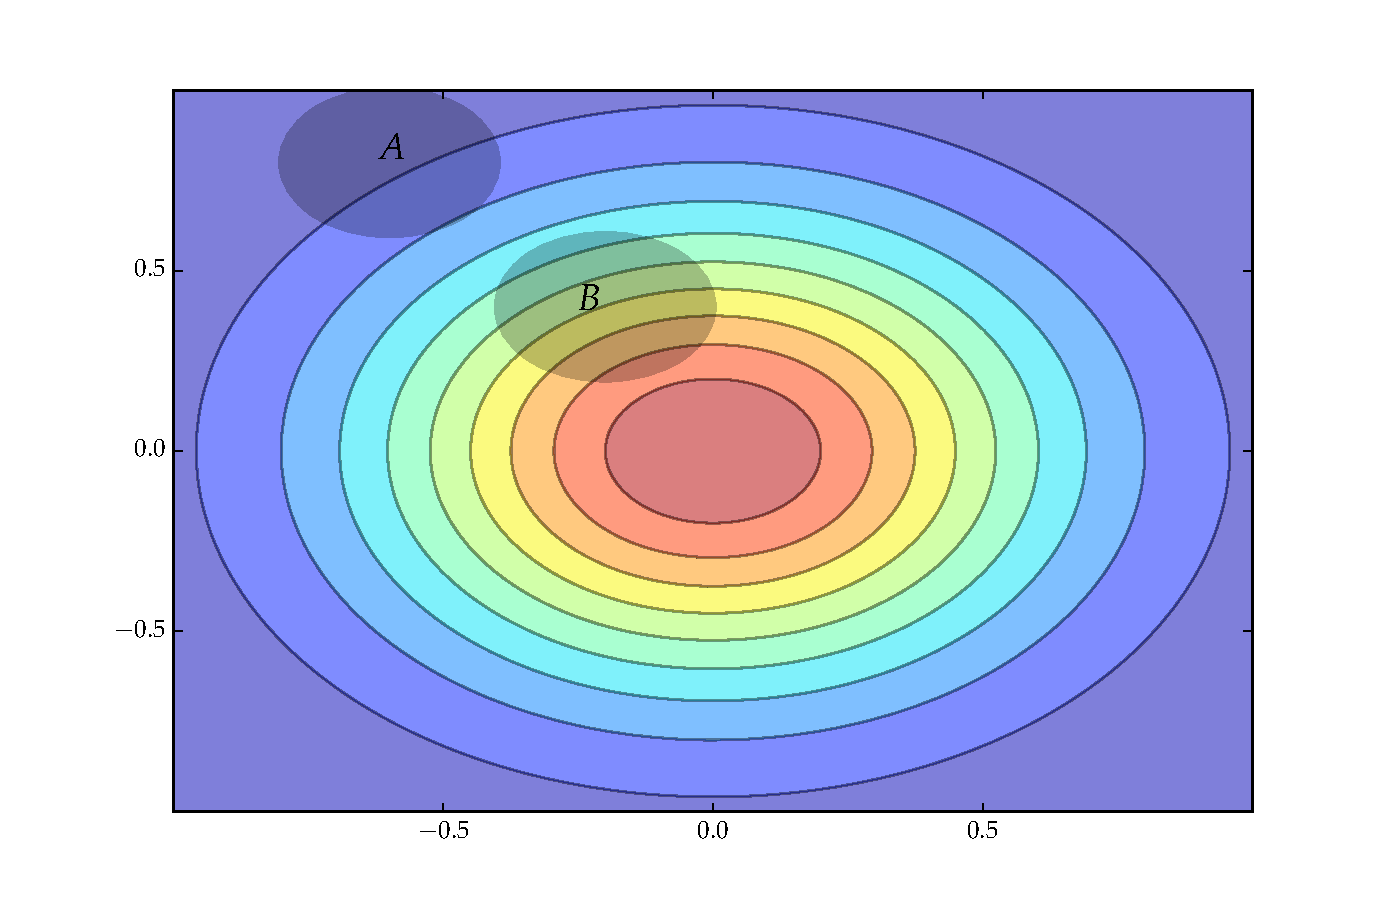
\includegraphics[trim={0 0em 0 2em}, clip]{gaussian_example.pdf}}
        \caption{\label{f:gaussian_example} Example distribution and events $A$ and $B$}
       \end{center}
    \end{figure}  

\end{frame}



\begin{frame}

    \vspace{2em}
    Any distribution $P$ on $\RR^N$ is characterised by the function 
    %
    \begin{equation*}
    \label{eq:ntf2}
    F(\bolds) :=
    F(s_1, \ldots, s_N) 
    := P \left( \times_{n=1}^N (-\infty, s_n] \right)
    \qquad (\bolds \in \RR^N)
    \end{equation*}
    
    The function $F$ is a \navy{multivariate cumulative distribution function},
    which is a function $F \colon \RR^N \to [0, 1]$ that is
    %
    \begin{enumerate}
            \label{enum:mcdf}
        \item right-continuous in each of its arguments,
        \item increasing in each of its arguments, and 
        \item satisfies
            %
            \begin{equation*}
                F(\bolds_j) \to 1 \text{ as }
                \bolds_j \to \infty 
                \quad 
            \end{equation*}
            \begin{equation*}
            \text{and} \quad
                F(s_1, \dots, s_{nj}, \dots, s_N) \to 0
                \text{ as }
                s_{nj} \to -\infty
            \end{equation*}
    \end{enumerate}
    
\end{frame}

\begin{frame}

    \vspace{2em}
     A distribution $P$ on $\RR^N$ is:
     %
     \begin{itemize}
         \item \navy{discrete} if $P$ is supported on a countable subset of $\RR^N$
         \item \navy{absolutely continuous} if $P(B) = 0$ whenever $B$ has zero Lebesgue measure
     \end{itemize}

\end{frame}

\begin{frame}
    
    \vspace{2em}
    Again, absolute continuity necessary and sufficient for existence of
    density representation:
    
    \begin{equation*}
    \label{eq:drbd3}
    P(B) = \int_B p(\bolds) \, \diff  \bolds
    \qquad \text{for all } B \in \bB(\RR^N)
    \end{equation*}
    
    \vspace{2em}
    The right-hand
    is a multivariate integral which we can write as
    %
    \begin{equation*}
        \label{eq:defjd0}
        \int_{-\infty}^{\infty}
            \cdots
            \int_{-\infty}^{\infty} 
            \1_B (s_1,\ldots,s_N)
            p(s_1,\ldots,s_N) 
            \diff s_1 \cdots \diff s_N
    \end{equation*}
    
    If $p$ is any density on $\RR^N$, then above defines a
    distribution
    
\end{frame}

\begin{frame}

    \vspace{2em}
    \Eg\label{eg:mnden}
    The \navy{multivariate normal density} or \navy{multivariate Gaussian density} on $\RR^N$
    is a function $p$ of the form
    %
    \begin{equation*}
        \label{eq:mnormden}
        p(\bolds) = (2 \pi)^{-N/2} \det(\boldSigma)^{-1/2} 
        \exp \left\{ 
            - \frac{1}{2} (\bolds - \boldmu)^\T \boldSigma^{-1} (\bolds - \boldmu) 
        \right\}
    \end{equation*}
    %
    where $\boldmu$ is any $N \times 1$ vector and $\boldSigma$ is a positive
    definite $N \times N$ matrix
    
    We represent this distribution
    by $\nN(\boldmu, \boldSigma)$
    
    \vspace{1em}
    The case $\nN(\boldzero, \boldI)$ is
    called the \navy{multivariate standard normal distribution}
    
\end{frame}

\begin{frame}

    \vspace{2em}
    \begin{figure}
    
   \centering
   \scalebox{.42}{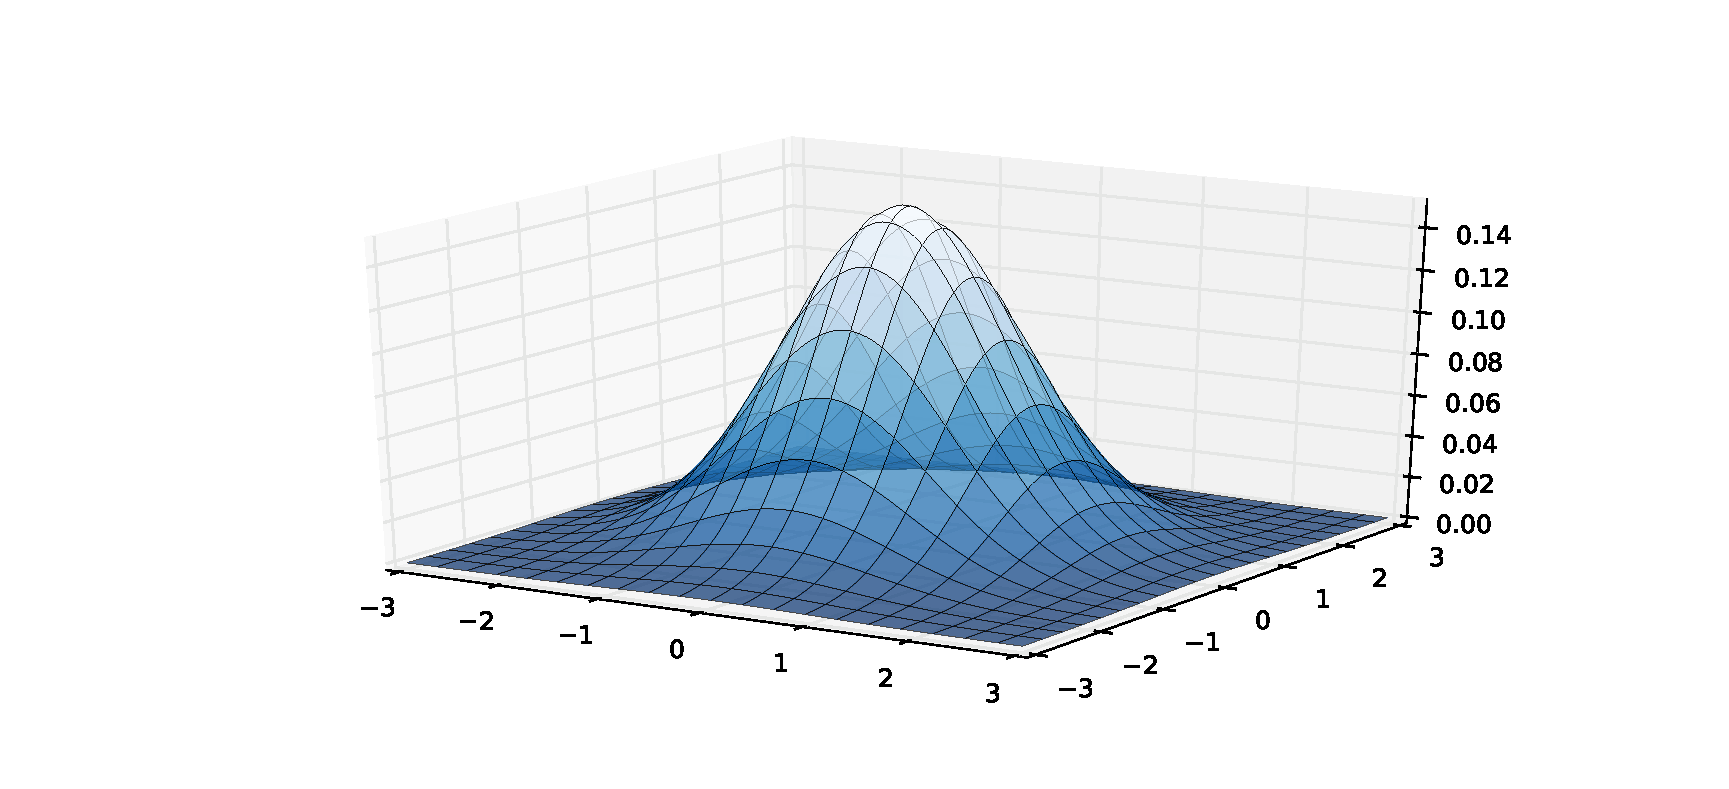
\includegraphics[trim={5em 5em 5em 5em}, clip]{bivar_gaussian_3d.pdf}}
   \caption{\label{f:bivar_gaussian_3d} Bivariate standard normal density}
   
    \end{figure}
    
\end{frame}
    
\begin{frame}
    
     \vspace{2em}
    The \navy{product distribution} of $P_1, \ldots,
    P_N$ is defined by the next fact:
    
     \vspace{1em}
    \Fact\eqref{ET-fa:prodist}
    Given distributions $P_1, \ldots, P_N$ on $\RR$, there exists a unique
    and well-defined distribution $\mathring{P}$ on $\RR^N$ such that
    %
    \begin{multline*}
        \mathring{P}(B_1 \times \cdots \times B_N)
        \\ = \prod_{n=1}^N P_n(B_n)
        \qquad \text{for all } B_n \in \bB(\RR), \; n=1,\ldots, N       
    \end{multline*}
    
    \vspace{1em}
    Unique because the distributions are uniquely pinned down by cylinder sets 
    of $\mathbb{R}^{N}$ (see page 128 in ET)
    
\end{frame}

\begin{frame}
    
    \vspace{2em}
    Given any distribution $P$ on $\RR^N$, the $n$th \navy{marginal
    distribution} of $P$ is the distribution on $\RR$ defined by 
    %
    \begin{equation*}
        P_n(B)
        = P (\RR \times \cdots \times \RR \times B \times \RR \times \cdots
        \times \RR)
    \end{equation*}
    
    \vspace{.7em}
    Here $B$ is the $n$th element of the Cartesian product
    
    \vspace{.7em}
    Equivalently, 
    %
    \begin{equation*}
    P_n(B) 
    = P \setntn{\bolds \in \RR^N}{\bolds^\T \bolde_n \in B}
    \end{equation*}
    
\end{frame}

\begin{frame}

    \vspace{2em}
    From $P_n$ we can also extract the \navy{marginal {\sc cdf} $F_n$} via 
    %
    \begin{equation*}
        \label{eq:ntf}
        F_{n}(s) := P_{n}( (-\infty, s] )
        \qquad (s \in \RR)
    \end{equation*}
    %
    (see page page~\pageref{ET-eq:ntf} of ET)
    
    \vspace{1em}
    If $P_n$ is absolutely continuous, it has density $p_n$
    
    When the joint
    distribution $P$ has a density $p$, the marginal distribution $P_n$ has a
    density $p_n$ -- ``integrate out
    other variables"
    
    \vspace{.7em}
    For example, the bivariate case:
    %
    \begin{equation*}
        p_1(s_1)
        = \int_{-\infty}^{\infty} p(s_1, s_2) \diff s_2
    \end{equation*}
    
\end{frame}

\begin{frame}
    
    \vspace{2em}
    \begin{figure}
       \begin{center}
        \scalebox{.44}{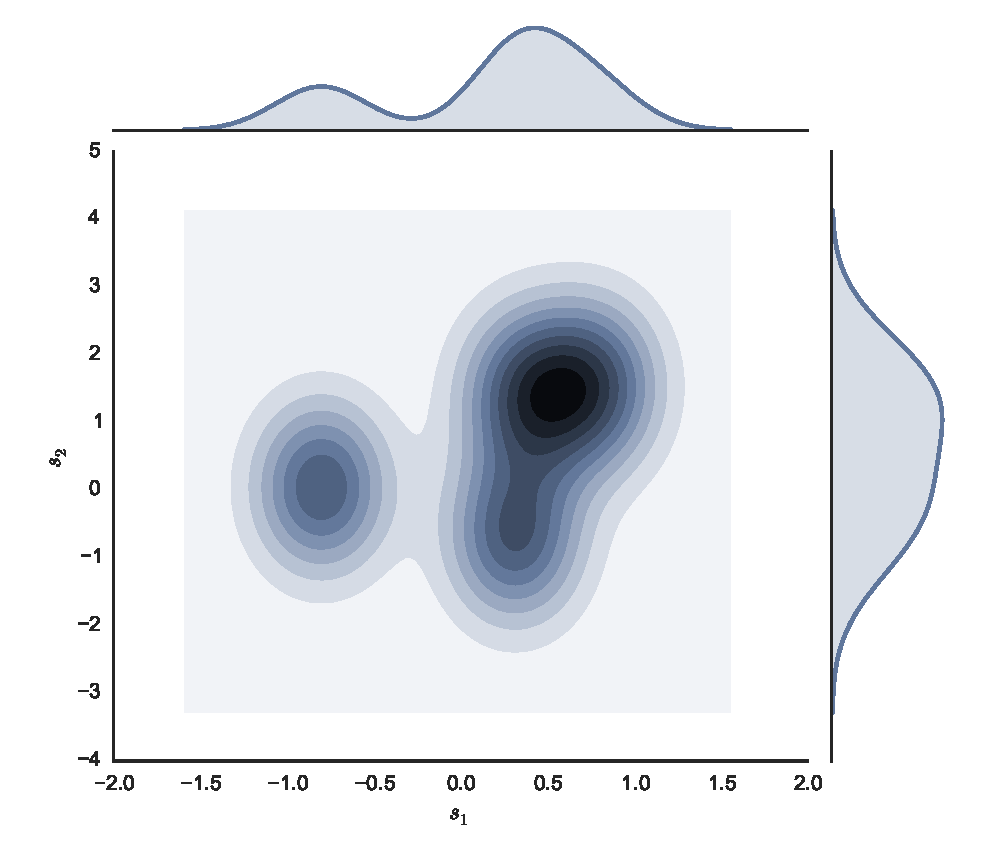
\includegraphics{jointplot.pdf}}
        \caption{\label{f:jointplot} Bivariate joint density and its two marginals}
       \end{center}
    \end{figure}
    
\end{frame}

\begin{frame}

    \vspace{2em}
    Joint distribution cannot be determined from the
    marginals alone
    \begin{itemize}
        \item marginals do not tell us
    about the interactions across coordinates
    \end{itemize} 
    
    \vspace{1em}
    The exception is 
    when there is no interaction -- the case for 
    product distributions 
    
\end{frame}

\begin{frame}\frametitle{Distributions of Random Vectors}
    
    \vspace{2em}
    Let $\boldx$ be a random vector in $\RR^N$
    
    \vspace{1em}
    The \navy{distribution} of
    $\boldx$ is the probability measure $P$ on $\bB(\RR^N)$ defined by
    %
    \begin{equation*}
        \label{eq:dmnu}
        P(B) = \PP\{\boldx \in B\}
        \qquad (B \in \bB(\RR^N))
    \end{equation*}
    %
    The $P$ here also called the \navy{joint distribution} of
    $x_1,\ldots, x_N$, and we write $\lL(\boldx) = P$
    
\end{frame}
    
\begin{frame}
    
    \vspace{2em}
    Joint distribution represented by the multivariate {\sc cdf} $F \colon \RR^N \to [0, 1]$:
    %
    $$F(s_1,\ldots,s_N) = \PP\{ x_1 \leq s_1, \ldots, x_N \leq s_N\}$$
    %
    or, in vector notation
    %
    \begin{equation*}
        F(\bolds) = \PP\{\boldx \leq \bolds\}
        \qquad (\bolds \in \RR^N)
    \end{equation*}
    
\end{frame}

\begin{frame}

    \vspace{2em}
    When the distribution $P$ of $\boldx$
    is absolutely continuous, there exists a non-negative function $p$ on $\RR^N$
    satisfying 
    %
    \begin{equation*}
        \label{eq:defjd00}
        \int_B p(\bolds) \diff  \bolds = \PP\{\boldx \in B\}
        \qquad (B \in \bB(\RR^N))
    \end{equation*}
    %
    The function $p$ is the \navy{joint density} of
    $\boldx$
    
    \vspace{1em}
    For the above to hold, it suffices that 
    \begin{equation*}
    \label{eq:defjd}
    \int_{-\infty}^{s_N} 
    \cdots
     \int_{-\infty}^{s_1} 
    p(t_1,\ldots,t_N) 
    \diff t_1 \cdots \diff t_N
    = F(s_1,\ldots,s_N) 
    \end{equation*}
    %
    for all $s_n  \in \RR$, $n=1,\ldots, N$ 
    
\end{frame}


\begin{frame}

    \vspace{2em}
    If $\boldx = (x_1,\ldots, x_N)$ is a random vector in $\RR^N$, then each $x_n$
    is a random variable on $\RR$
    
    \vspace{1em}
    Let $P_n = \lL(x_n)$, so: 
    %
    \begin{equation*}
        \label{eq:deffx2}
        P_n(B) = \PP \{x_n \in B \}
        \qquad (B \in \bB(\RR), \; n = 1, \ldots, N)
    \end{equation*}
    %

    $P_n$ is called
    the \navy{marginal distribution of $x_n$}
    
    If $P_1 = P_2 = \cdots = P_N$, then $x_1, \ldots, x_N$ are \navy{identically distributed}
    
\end{frame}

\begin{frame}\frametitle{Gaussian Random Vectors}
    
    \vspace{2em}
    A random variable $x$ is
    \navy{normally distributed} if $x = \mu + \sigma z$ for some $\sigma \geq 0$
    
    We write $\lL(x) = \nN(\mu, \sigma)$
    
\end{frame}

\begin{frame}
    
    \vspace{2em}
    A random vector $\boldx$ in $\RR^N$ is \navy{multivariate normal} or \navy{multivariate Gaussian} if
    %
    \begin{equation*}
        \label{eq:imn}
        \boldx = \boldmu + \boldC \boldz
    \end{equation*}
    %
    where the term $\boldz$ is a $K \times 1$ standard normal
    random vector, the matrix $\boldC$ is $N \times K$ and the vector $\boldmu$  is $N \times 1$
    
    \vspace{1em}
    If $\boldx$ is multivariate normal, then we write $\lL(\boldx ) =
    \nN(\boldmu, \boldSigma)$, where
    %
    \begin{equation*}
        \boldmu := \EE \boldx 
        \quad \text{and} \quad
        \boldSigma := \var \boldx
    \end{equation*}
    %
    We have $\boldSigma = \boldC\boldC^\T$ (recall fact 5.1.2 in ET)
    
\end{frame}

\begin{frame}
    
    \vspace{2em}
   $\lL(\boldx) = \nN(\boldmu, \boldSigma)$ does not imply
    $\boldx$ has the multivariate normal density
    \begin{itemize}
        \item distribution of $\boldx$ can fail to be absolutely
            continuous for e.g. if $\boldC = \boldzero$ 
    \end{itemize}
    
    \vspace{1em}
    Absolute continuity of the distribution of $\boldx$ coincides with 
    the setting where $\boldSigma := \var \boldx$ is nonsingular -- 
    nonsingularity of $\boldSigma$ will be true if and only if
    $\boldC^\T$ has full column rank
    
\end{frame}

\begin{frame}
    
    \vspace{2em}
    \Fact\eqref{ET-fa:nipre}
    Let $\boldx$ be a random vector in $\RR^N$.  The following statements are true:
    %
    \begin{enumerate}
        \item The vector $\boldx$ is multivariate normal  if and only if
            $\bolda^\T \boldx$ is normally distributed in $\RR$ for every
            constant $N \times 1$ vector $\bolda$
        \item If $\lL(\boldx) = \nN(\boldmu, \boldSigma)$, then 
            %
            \begin{equation*}
                  \lL(\boldA \boldx + \boldb) = \nN(\boldA \boldmu + \boldb, \boldA
                    \boldSigma \boldA^\T)  
            \end{equation*}
            %
            for all constant conformable $\boldA, \boldb$
    \end{enumerate}
    
\end{frame}

\begin{frame}

    \vspace{2em}
    Corollary: if $\boldx = (x_1,
    \ldots, x_N)$ is multivariate normal, then the marginal distribution of 
    $x_n$ is univariate normal
    
    Is the
    joint distribution of $N$ univariate normal random variables always
    multivariate normal? 
    \begin{itemize}
        \item Answer: no
    \end{itemize}
    
\end{frame}

\begin{frame}\frametitle{Expectations from Distributions}

    \vspace{2em}
    Let $h \colon \RR^N \to \RR$ be any $\bB$-measurable function and let
    $P$ be a distribution on $\RR^N$
    
    The function $h$ now regarded as a random variable on 
    $(\RR^N, \bB(\RR^N), P)$
    
    Expectation of $h$ can be writen as
    %
    \begin{equation}
        \label{eq:eph}
        \EEP h :=: \int h(\bolds) P(\diff \bolds)
    \end{equation}
    
\end{frame}

\begin{frame}

    \vspace{2em}
    \Fact\eqref{ET-fa:haspvec}
        Let $h \colon \RR^N \to \RR$ be $\bB$-measurable and let $P$ be a
        distribution on $\RR^N$.  If $P$ is discrete, with {\sc pmf} $\{p_j\}_{j
        \geq 1}$ and support $\{\bolds_j\}_{j \geq 1}$, then
        %
        \begin{equation}
            \label{eq:hasp2}
            \int h(\bolds) P(\diff \bolds) = \sum_{j\geq 1} h(\bolds_j) p_j 
        \end{equation}
        %
        If $P$ is absolutely continuous with density $p$, then
        %
        \begin{equation}
            \label{eq:hasd2}
            \int h(\bolds)P(\diff \bolds) 
            = \int h(\bolds) p(\bolds) \diff \bolds
    \end{equation}
    
    The right-hand side of \eqref{eq:hasd2} should be understood as 
    %
    \begin{equation*}
        \int_{-\infty}^\infty
            \cdots
            \int_{-\infty}^\infty
            h(s_1, \ldots, s_N) \,
            p(s_1,\ldots,s_N)  \,
            \diff s_1 \cdots \diff s_N
    \end{equation*}
    %
\end{frame}

\begin{frame}
    
    \vspace{2em}
    As in the univariate case, objects like moments are properties
    of the distribution

    \vspace{1em}
    For example, let $\boldx$ be a random vector in $\RR^K$
    with $\lL(\boldx) = P$
    
    The variance--covariance matrix $\var [\boldx]$ of
    $\boldx$ has $i,j$th element $\EE [x_i x_j] - \EE[x_i]\EE[x_j]$
    
    We can
    write $\var [\boldx]$ in terms of $P$. If
    %
    \begin{equation*}
        \label{eq:vcd2}
        \boldSigma_P = (\sigma_{ij}) 
        \quad \text{where} \quad
        \sigma_{ij} := \int (s_i s_j) P(\diff \bolds) 
            - \int s_i P(\diff \bolds) \cdot \int s_j P(\diff \bolds)
    \end{equation*}
    %
    then $\boldSigma_P = \var[\boldx]$
    
\end{frame}

\begin{frame}\frametitle{Independence of Random Variables}

    \vspace{2em}
    A collection of $N$ random variables $x_1, \ldots, x_N$ is \navy{independent} if
    %
    \begin{equation}
        \label{eq:bcap}
        \PP \bigcap_{n=1}^N \{x_n \in B_n\}
        = \prod_{n=1}^N \PP\{x_n \in B_n\} 
    \end{equation}
    %
    for any $B_1, \ldots, B_N$, where each $B_n$ is a Borel subset of $\RR$
    
    \vspace{1em}
    The random variables $x_1, \ldots, x_N$ are
    independent when sets of the form $\{x_1 \in B_1\}, \ldots, \{x_N
    \in B_N\}$ are independent events
    
    An infinite set of random variables $\{x_n\}_{n=1}^{\infty}$ is
    independent if any finite subset of $\{x_n\}_{n=1}^{\infty}$ is independent
    
\end{frame}

\begin{frame}

    \vspace{2em}
    Equivalent definition of independence using distributions
    
    Let $P$ be the joint distribution of $\boldx = (x_1, \ldots, x_N)$ and $P_n$ be its $n$th marginal
    
    Since
    $\cap_{n=1}^N \{x_n \in B_n\}
    = \{ (x_1, \ldots, x_N) \in B_1 \times \cdots \times B_N \}$, the random
    variables $x_1, \ldots, x_N$ are independent if
    %
    \begin{equation*}
        P(B_1 \times \cdots \times B_N) 
        = \prod_{n=1}^N P_n(B_n)
    \end{equation*}
    
    Elements of a random vector are
    independent if and only if their joint distribution equals 
    the product distribution formed from their marginals 
    
\end{frame}

\begin{frame}

    \vspace{2em}
    A necessary and sufficient condition for independence of $x_1,
    \ldots, x_N$ is:
    %
    \begin{equation*}
        \label{eq:pdind}
        F(s_1,\ldots,s_N) 
        = \prod_{n=1}^N F_n(s_n)
    \end{equation*}
    %
    for all $(s_1, \ldots, s_N) \in \RR^N$, where $F$ is the {\sc cdf} of $\boldx$ and
    $F_1, \ldots, F_N$ are the marginal {\sc cdf}s (why?)
    
\end{frame}

\begin{frame}
    
    \vspace{2em}
    If the distribution of $\boldx$ is absolutely continuous we can also test
    independence via its density: 
    
    \vspace{1em}
    \Fact\eqref{ET-fa:immd}
        If $\boldx = (x_1, \ldots, x_N)$ has joint density $p$ and marginals
        $p_1, \ldots, p_N$, then $x_1, \ldots, x_N$ are independent if and only if
        %
        \begin{equation*}
            p (s_1,\ldots, s_N) = \prod_{n=1}^N p_n(s_n)
            \qquad \text{for all} \quad
            (s_1, \ldots, s_N) \in \RR^N
        \end{equation*}
        
\end{frame}

\begin{frame}

    \vspace{2em}
    \Eg 
    
    Let $\lL(\boldx) = \lL(x_1, \ldots, x_N) = N(\boldmu, \boldSigma)$ 
    
    Suppose in
    addition that $\boldSigma$ is diagonal, with $n$th diagonal component
    $\sigma_n > 0$, then $x_1, \ldots, x_N$ are independent
    
    To see this, observe for any
    $\bolds = (s_1, \ldots, s_N) \in \RR^N$, we have
    %
    \begin{align*}
        p(\bolds) 
        & = (2 \pi)^{-N/2} \determinant (\boldSigma)^{-1/2} 
        \exp \left\{ 
            - \frac{1}{2} (\bolds - \boldmu)^\T \boldSigma^{-1} (\bolds - \boldmu) 
        \right\}
        \\
        & = \frac{1}{(2 \pi)^{N/2} \prod_{n=1}^N \sigma_n}
        \exp \left\{ 
            - \frac{1}{2} \sum_{n=1}^N (s_n - \mu_n)^2 \sigma_n^{-2}
        \right\}
    \end{align*}
    
\end{frame}

\begin{frame}

    \vspace{2em}
    \Eg (cont.)
    Computation of the determinant and inverse of $\boldSigma$ used 
    facts~\ref{ET-fa:dtmat} and \ref{ET-fa:powdm}
    
    The last expression can be factored further
    %
    \begin{equation*}
        p(\bolds) 
        =
        \prod_{n=1}^N \frac{1}{(2 \pi)^{1/2} \sigma_n}
            \exp \left\{ 
                \frac{-(s_n - \mu_n)^2}{2 \sigma_n^2}
            \right\}
         =
        \prod_{n=1}^N p_n(s_n)
    \end{equation*}
    %
    where $p_n$ is the density of $\nN(\mu_n, \sigma^2_n)$

\end{frame}

\begin{frame}

    \vspace{2em}
    \Fact\eqref{ET-fa:imme}
   If $x_1, \ldots, x_N$ are independent and each $x_n$ is integrable, then
   %
   \begin{equation*}
       \EE \left[ \prod_{n=1}^N x_n \right]
       = \prod_{n=1}^N \EE[ x_n ]
   \end{equation*}
   %
\end{frame}

\begin{frame}\frametitle{Independence of Random Vectors}

    \vspace{2em}
    Random vectors $\boldx_1, \ldots, \boldx_N$ in $\RR^K$ are called
    \navy{independent} if
    %
    \begin{equation*}
        \label{eq:bcapv}
        \PP \bigcap_{n=1}^N \{\boldx_n \in B_n\}
        = \prod_{n=1}^N \PP\{\boldx_n \in B_n\} 
    \end{equation*}
    %
    for any $B_1, \ldots, B_N$, where each $B_n$ is a Borel subset of $\RR^K$
    
\end{frame}

\begin{frame}
    
    \vspace{2em}
    \Fact\eqref{ET-fa:rviifi}
    If $\boldx_1, \ldots, \boldx_N$ are independent random vectors in $\RR^K$ and 
    $f_1, \ldots, f_N$ are any $\bB$-measurable functions,
    then $f_1(\boldx_1), \ldots, f_N(\boldx_N)$ are also independent.
    
    \Prf 
    Observe  $f_n(\boldx_n) \in B_n$ if and only if $\boldx_n \in
    f^{-1}(B_n)$. This leads to 
    %
    \begin{equation*}
        \bigcap_{n=1}^N \{f_n(\boldx_n) \in B_n\}
        = \bigcap_{n=1}^N \{\boldx_n \in f^{-1}(B_n)\}
    \end{equation*}
    %
    Applying independence of $\boldx_1, \ldots, \boldx_N$
    %
    \begin{multline*}
        \PP
        \bigcap_{n=1}^N \{f_n(\boldx_n) \in B_n\}
        \\ = \prod_{n=1}^N \PP \{\boldx_n \in f^{-1}(B_n)\}
        = \prod_{n=1}^N \PP \{f_n(\boldx_n) \in B_n\}
    \end{multline*}
    %
    
\end{frame}

\begin{frame}

    \vspace{2em}
    \Fact\eqref{ET-fa:indzcov}
    If $\boldx$ and $\boldy$ are independent, then $\cov(\boldx,\boldy) = 0$.
        
    Converse not true:  one can construct examples of dependent
    random variables with zero covariance.  However,

    \Fact\eqref{ET-fa:ucimin}
    If $\boldx$ is multivariate Gaussian and $\boldA$ and $\boldB$ are
    conformable constant matrices, then $\boldA \boldx$ and
    $\boldB \boldx$ are independent if and only if $\cov(\boldA \boldx, \boldB\boldx) = \boldzero$
        
\end{frame}

\begin{frame}

    \vspace{2em}
    \Fact\eqref{ET-fa:poci}
    Let $S$ be any linear subspace of $\RR^N$, let $\boldP := \proj S$ and let
    $\boldM$ be the residual projection.  If $\lL(\boldz) = \nN(\boldzero,
    \sigma^2 \boldI)$ in $\RR^N$ for some $\sigma^2 > 0$, then $\boldP \boldz$ and
    $\boldM \boldz$ are independent
    
    \vspace{1em}
    \Fact\eqref{ET-fa:lcinorm}
        If $w_1, \ldots, w_N$ are independent with $\lL(w_n) = \nN(\mu_n,
        \sigma_n^2)$ for all $n$, then
        %
        \begin{equation*}
            \lL \left[ \alpha_0 + \sum_{n=1}^N \alpha_n w_n \right]
            = \nN \left( 
                \alpha_0 + \sum_{n=1}^N \alpha_n \mu_n,\;
                \sum_{n=1}^N \alpha_n^2 \sigma_n^2
                \right)
        \end{equation*}
        %
\end{frame}

\begin{frame}

    \vspace{1em}
    Sums of arbitrary normals are not always normal --- we require a multivariate
    normal distribution
    
    \vspace{1em}
    In fact \eqref{ET-fa:lcinorm} above:
    %
    $$\lL(w_1, \ldots, w_N) = \nN(\boldmu,
    \boldSigma)$$ 
    %
    where $\bolde_n^\T \, \boldmu = \mu_n$, and
    %
    $$\boldSigma =
    \diag(\sigma_1^2, \ldots, \sigma_N^2)$$
 
    
\end{frame}

\section{Copulas}

\begin{frame}

    \vspace{2em}
    A \navy{copula} $C$ on $\RR^N$ is a multivariate {\sc cdf} supported
    on the unit hypercube $[0, 1]^N$ with the
    property that all its marginals are uniform on $[0, 1]$
    
    $C$ is a function of the form
    %
    \begin{equation}
        \label{eq:icif}
        C(s_1, \ldots, s_N) = \PP \{u_1 \leq s_1, \ldots, u_N \leq s_N\}
    \end{equation}
    %
    Where $0 \leq s_n \leq 1$ and $\lL(u_n) = U[0, 1]$ for all $n$
    
    \vspace{1em}
    While each $u_n$ has its marginal
    distribution pinned down, there are infinitely many ways to specify the joint distribution
        
\end{frame}

\begin{frame}

    \vspace{2em}
    \Eg The function $C(s_1, s_2) = s_1 s_2$ on $[0, 1]^2$ is called the
    \navy{independence copula}
    
    \vspace{1em}
    The marginal distributions are $C(s_1, 1) =
    s_1$ and $C(1, s_2) = s_2$ as required
    
    (These are {\sc cdf}s for the
    $U[0, 1]$ distribution.)

\end{frame}

\begin{frame}

    \vspace{2em}
    \Eg
    The \navy{Gumbel copulas} are the class of functions on $[0, 1]^2$ defined by
    %
    \begin{equation*}
        C(s_1, s_2) = 
        \exp 
        \left\{
            - \left[ 
                (-\ln s_1)^\theta + (-\ln s_2)^\theta
            \right]^{1/\theta}
        \right\}
        , \quad (\theta \geq 1)
    \end{equation*}
    %
    The \navy{Clayton copulas} are given by
    %
    \begin{equation*}
        C(s_1, s_2) = 
        \left\{
            \max \left[
                s_1^{-\theta} +  s_2^{-\theta} -1, \, 0
                \right]
        \right\}^{-1/\theta}
        ,\quad (\theta \geq -1, \, \theta \not= 0)
    \end{equation*}
   
    Both of these belong to a general class called the \navy{Archimedean copulas}

\end{frame}

\begin{frame}

    \vspace{2em}
    We can take univariate {\sc cdf}s
    $F_1, \ldots, F_N$ and a copula $C$ to create a multivariate {\sc cdf} on
    $\RR^N$ via
    %
    \begin{multline}
        \label{eq:ffcop}
        F(s_1, \ldots, s_N) = C(F_1(s_1), \ldots, F_N(s_N))
        \\ (s_n \in \RR, \, n=1, \ldots, N)
    \end{multline}
    
    \vspace{1em}
    Benefit: separate out
    specification of the marginals and specification of the joint distribution
    
\end{frame}

\begin{frame}

    \vspace{2em}
    \Eg
    \cite{bonhomme2009assessing} use copulas to model one component of
    earnings dynamics in a study based on three-year panels from the French
    Labor Force Survey
    
    The cross sections are relatively large (around
    30,000), allowing for flexible modeling of the marginal distributions via
    a mixture of normals
    
    However, the time series dimension is
    short, so a one-parameter family of copulas is used to bind the
    marginals across time in a parsimonious way

\end{frame}

\begin{frame}

    \vspace{2em}
    \Thm\eqref{ET-t:sklar}
        If $F$ is any {\sc cdf} on $\RR^N$ with marginals $F_1, \ldots, F_N$,
        then there exists a copula $C$ such that \eqref{eq:ffcop} holds.  If each
        $F_n$ is continuous, then this representation is unique.
        
\end{frame}

\begin{frame}

    \vspace{2em}
    If $F_1, \ldots, F_N$ are univariate normal, then $C(F_1(s_1), \ldots, F_N(s_N))$
    will equal the multivariate normal {\sc cdf} for one choice of copula,
    called the Gaussian copula
    
    \vspace{2em}
    Other choices lead to different distributions
    
\end{frame}

\begin{frame}
    
    \vspace{2em}
    \begin{figure}
       \centering
       \scalebox{.44}{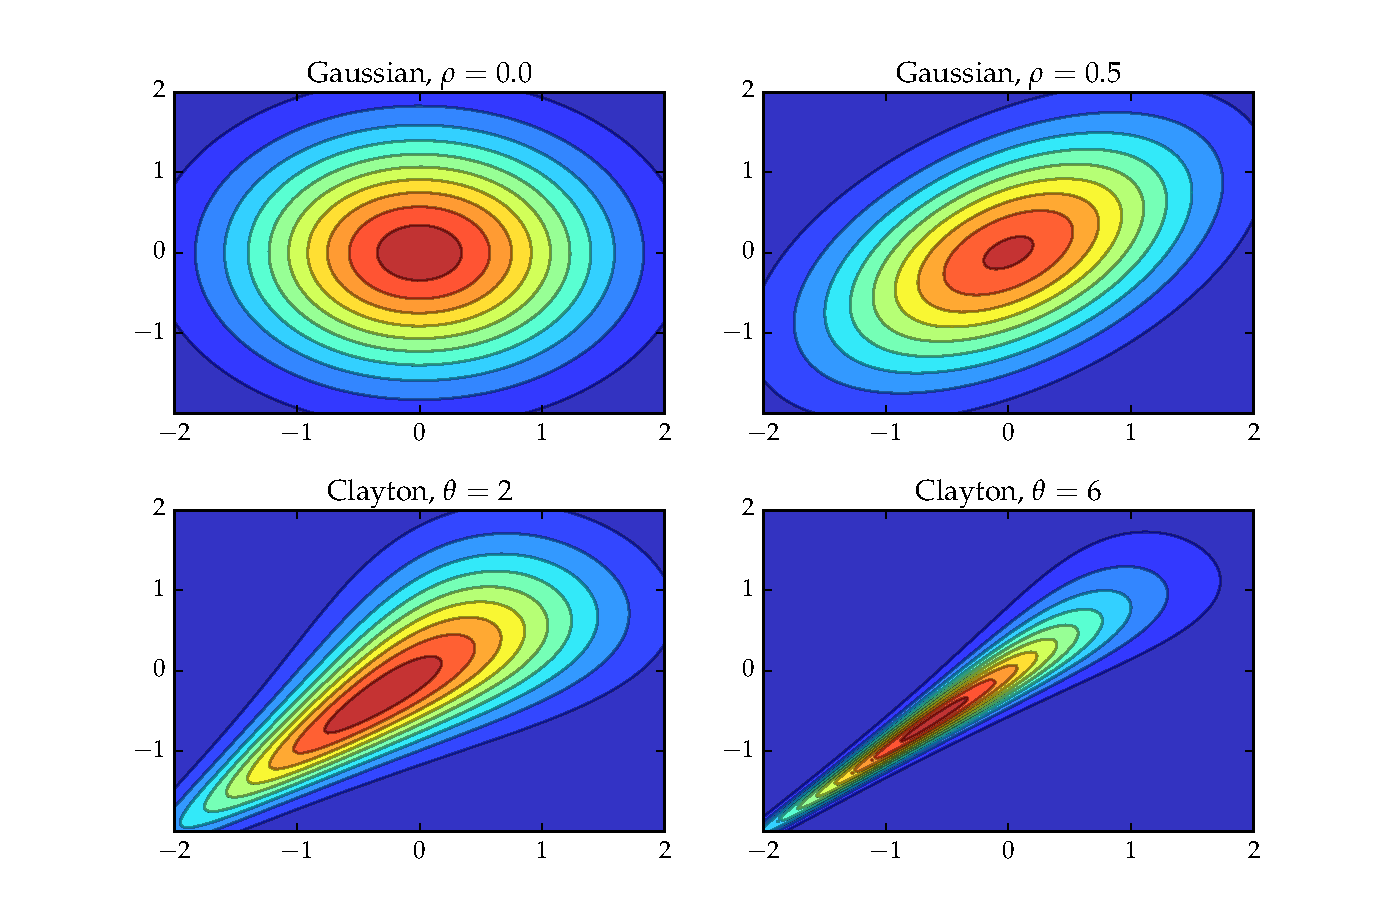
\includegraphics[trim={0 2em 0 2em}, clip]{copula.pdf}}
       \caption{\label{f:copula} Bivariate Gaussian (top) and non-Gaussian (bottom)}
    \end{figure}
    
\end{frame}

\section{Properties of Named Distributions}

\begin{frame}\frametitle{Properties of Named Distribution}

    \vspace{2em}
    \Fact
    \eqref{ET-fa:schis}
    If $x_1,\ldots,x_N$ are independent and $\lL(x_n) = \chi^2(k_n)$,
     then $\lL(\sum_n x_n) = \chi^2(\sum_n k_n)$
    
    \vspace{2em}
    \Fact
    \eqref{ET-fa:astudt}
    If $z$ and $x$ are independent with $\lL(z) = \nN(0,1)$ and $\lL(x) = \chi^2(k)$, 
    then 
    %
    \begin{equation*}
        z \sqrt{\frac{k}{x} } 
        \;\;
        \text{ is $t$ distributed with $k$ degrees of freedom}
    \end{equation*}
    

\end{frame}

\begin{frame}

    \vspace{2em}
    \Fact
    \eqref{ET-fa:ssnac}
    If $\lL(z_1, \ldots, z_N) = \nN(\boldzero, \boldI)$, then
    $\lL(\sum_{n=1}^N z_n^2) = \chi^2(N)$. 
    
    \vspace{2em}
    \Fact
    \eqref{ET-fa:mcfi}
    If $\lL(\boldz) = \nN(\boldzero, \boldI)$ and $\boldA$ is symmetric and
    idempotent, then 
    %
    \begin{equation*}
        \lL \left( \boldz^\T \boldA \boldz \right) = \chi^2(K)  
        \quad \text{where} \quad
        K := \trace \boldA
    \end{equation*}
    
    \vspace{1em}
    Exercise: obtain Fact \eqref{ET-fa:mcfi} from Fact \eqref{ET-fa:ssnac}.
    (See page~\pageref{ET-fa:mcfi} in eT)
    
\end{frame}

\section{Conditioning and Expectation}

\begin{frame}\frametitle{Conditioning and Expectation}

    \vspace{2em}
    Conditional expectation is one of the most important concepts in
    both economic theory and econometrics
    
    This section gives a construction of 
    expectation based around projection:
    
    \begin{itemize}
        \item frame conditional expectation as optimal
        prediction given limited information
    \end{itemize}

\end{frame}

\begin{frame}\frametitle{Conditional Densities}

    \vspace{2em}
    First some discussion of conditional densities 
    
    Let $x_1$ and $x_2$ be random variables.  The \navy{conditional density} 
    of $x_2$ given $x_1 = s_1$ is defined as 
    %
    \begin{equation*}
        p(s_2 \given s_1) 
            := \frac{p(s_1, s_2)}{p(s_2)}
    \end{equation*}
    
    Here $p$ stands in for either joint, marginal, or conditional density, 
    with the type determined by the argument
    
\end{frame}

\begin{frame}

    \vspace{2em}
    The law of total probability extends to the
    density case as follows: If $(x_1, x_2)$ is a random vector on $\RR^2$, then
    %
    \begin{equation*}
        \label{eq:dltp}
        p(s_2)
        = \int_{-\infty}^{\infty} p(s_2 \given s_1) p(s_1) \diff s_1
        \qquad \qquad 
        (s_2 \in \RR)
    \end{equation*}
    
    \Prf 
    To see this, fix $s_2 \in \RR$ and integrate the joint density to get the marginal, giving
    %
    $$
        p(s_2) = \int_{-\infty}^{\infty} p(s_1, s_2) \diff s_1
    $$
    Combine with $p(s_2 \given s_1) = p(s_1, s_2)/p(s_1)$ to yield the result
    
\end{frame}

\begin{frame}

    \vspace{2em}
    Bayes' law also extends to the
    density case:
    %
    \begin{equation*}
        \label{eq:brdc}
        p(s_2 \given s_1) = \frac{p(s_1 \given s_2) p(s_2)}{p(s_1)}
    \end{equation*}

\end{frame}

\begin{frame}

    \vspace{2em}
    The conditional density of $x_{k+1},\ldots, x_N$ given $x_1 = s_1,\ldots, x_k =
    s_k$ is defined by
    %
    \begin{equation*}
        \label{eq:condden}
        p(s_{k+1},\ldots,s_N \given s_1,\ldots,s_k) 
            = \frac{p(s_1,\ldots,s_N)}{p(s_1,\ldots,s_k)}
    \end{equation*}
    
    \vspace{1em}
    Rearrange to obtain a useful decomposition of the joint
    density:
    %
    \begin{equation*}
        \label{eq:decompjd}
        p(s_1,\ldots,s_N) 
        = p(s_{k+1},\ldots,s_N \given s_1,\ldots,s_k) p(s_1,\ldots,s_k)
    \end{equation*}
    
\end{frame}

\begin{frame}

    \vspace{2em}
    Suppose we want to predict random variable $y$ using another variable $x$
    
    Choose $x$ such that $x$ and $y$ are expected to be close
    under most realizations of uncertainty
    
    \vspace{1em}
    But what does ``expected to be close" mean?
    
\end{frame}

\begin{frame}

    \vspace{2em}
    The \navy{mean squared error} (MSE)
    $$\EE [ (x -
    y)^2 ]$$
    
    The \navy{root mean squared
    error}:
    %
    \begin{equation}
        \label{eq:ndrv}
        \| x - y \| := \sqrt{ \EE [ (x - y)^2 ] }
    \end{equation}
    
    There are many parallels between ordinary
    vector space with the Euclidean norm and the set of random variables  combined
    with the ``norm" defined in \eqref{eq:ndrv} --- we formalise these ideas next 
    
\end{frame}

\begin{frame}

    \vspace{2em}
    The first geometric concept we defined for vectors was inner product
    
    Analogously, define the \navy{inner product between two random
    variables} $x$ and $y$
    %
    \begin{equation*}
        \label{eq:ipl2}
        \inner{x, y} := \EE[xy]
    \end{equation*}
    
    \vspace{1em}
    Cauchy--Schwarz
    inequality for random variables tells us
    $\EE[xy]$ will
    be finite and well-defined whenever $x$ and $y$ both have finite second
    moments
    
\end{frame}

\begin{frame}
    
    \vspace{2em}
    The set of random variables with finite second moments commonly denoted as $L_2$ 
    %
    \begin{equation*}
        L_2 
        := \{ \text{ all random variables } x \text{ on } (\Omega, \fF, \PP)
        \text{ with } \EE [x^2] < \infty \}
    \end{equation*}

    \Fact\eqref{ET-fa:innpp2}
    For any $\alpha, \beta \in \RR$ and any $x, y, z \in L_2$, the following 
    statements are true:
    %
    \begin{enumerate}
        \item $\inner{x, y} = \inner{y, x}$.
        \item $\inner{\alpha x, \beta y} =  \alpha \beta \inner{x, y}$.
        \item $\inner{x, \alpha y + \beta z} =  \alpha
            \inner{x, y} + \beta \inner{x, z}$.
    \end{enumerate}
    %
    Properties  follow from the definition of the inner product and linearity of $\EE$
    
    Compare above with Fact~\ref{ET-fa:innpp} in ET for vectors in Euclidean space 
    
\end{frame}

\begin{frame}

    \vspace{2em}
    Define the \navy{$L_2$ norm} by
    %
    \begin{equation*}
        \label{eq:rvnorm}
        \| x \| 
        := \sqrt{ \inner{x, x} } 
        := \sqrt{ \EE[x^2] } 
        \qquad (x \in L_2)
    \end{equation*}
    
    Norm gives notion of distance $\|x - y\|$ between random
    variables that agrees with the notion of root MSE
    
    \vspace{1em}
    \Fact\eqref{ET-fa:l2se}
    For any $\alpha \in \RR$ and any $x, y \in L_2$, the following 
    statements are true:
    %
    \begin{enumerate}
        \item $\| x \| \geq 0$ and $\| x \| = 0$ if and only if
            $x = 0$
        \item $\| \alpha x \| = |\alpha| \| x \|$
        \item $\| x + y \| \leq  \| x \| + \| y \|$
        \item $| \! \inner{x, y}\!  | \leq  \| x \| \| y \|$
    \end{enumerate}
    
\end{frame}

\begin{frame}

    \vspace{2em}
    Property 2. of above fact is
    immediate from definition of norm and the linearity of $\EE$
    
    Property 3.
    is called the \navy{triangle inequality}, as in the vector case
    
    Property
    4. is just the \navy{Cauchy--Schwarz inequality} for random variables from
    page~\pageref{ET-fa:csrv}
    
    As in the vector case, the
    triangle inequality can be proved from the Cauchy--Schwarz inequality (see exercise~\ref{ET-ex:csrv})
    
\end{frame}

\begin{frame}

    \vspace{2em}
    Regarding 1., it isn't true that $\| x \| = 0$ implies $x(\omega) = 0$ for all $\omega \in \Omega$
    
    What we can say is that if $\| x \| = 0$, then
    $\PP\{x =0\} =1$
    
    \vspace{1em}
    In dealing with  with $L_2$, convention to not distinguish between random variables that only differ with zero
    probability
    
\end{frame}

\begin{frame}\frametitle{Linear Subspaces in $L_2$}

    \vspace{2em}
    Any \navy{linear combination}  of random variables with finite variance
    
    \begin{equation}
        \alpha_1 x_1 + \cdots \alpha_K x_K,
        \qquad \alpha_k \in \RR, \; x_k \in L_2
    \end{equation}
    %
    is again in $L_2$
    
    When $X$ is a subset of $L_2$, the set of finite linear
    combinations that can be formed from elements of $X$ is called the \navy{span}
    of $X$, and denoted by $\Span X$
    
\end{frame}

\begin{frame}

    \vspace{2em}
    \Eg
    If $x \in L_2$ and $\1 := \1_\Omega$ is the constant random variable 
    always equal to $1$, then $\Span\{\1, x\}$ is the set of random variables
    %
    \begin{equation}
        \label{eq:llasp}
         \alpha + \beta x 
         := \alpha \1 + \beta x
         \quad \text{for scalars} \quad
         \alpha, \beta   
    \end{equation}
    %
    This is the set $\lL$ introduced from when we
    discussed best linear predictors
    
\end{frame}

\begin{frame}

    \vspace{2em}
    A subset $S$ of $L_2$ is called a
    \navy{linear subspace} of $L_2$ if it is closed under addition and scalar
    multiplication
    \begin{itemize}
        \item for each $x, y \in S$ and $\alpha, \beta \in \RR$,
    we have $\alpha x + \beta y \in S$
    \end{itemize}

    \vspace{1em}
    \Eg
    The span of any set of elements of $L_2$ is a linear subspace in $L_2$

\end{frame}

\begin{frame}

    \vspace{2em}
    \Eg
    The set $Z := \setntn{x \in L_2}{\EE x = 0}$ is 
    a linear subspace of $L_2$ because 
    %
    \begin{equation*}
        x, y \in Z
        \text{ and }
        \alpha, \beta \in \RR
         \implies
        \EE[\alpha x + \beta y] = \alpha \EE[x] + \beta \EE[y] = 0
    \end{equation*}
    
    \vspace{1em}    
    As in $\RR^N$, an \navy{orthonormal basis} of a linear subspace $S$ of $L_2$ 
    is a set $\{u_1, \ldots, u_K\} \subset S$ with the property 
    %
    \begin{align*}
        \inner{u_j, u_k}  = \1\{j = k\}
       \\  \quad \text{and} \quad
        \Span\{u_1, \ldots, u_K\} = S
    \end{align*}

\end{frame}

\begin{frame}

    \vspace{2em}
    \Eg
    Let $x \in L_2$ so that $S := \Span\{\1, x\}$ is the set of random variables
    %
    \begin{equation}
         \alpha + \beta x 
         := \alpha \1 + \beta x
         \quad \text{for scalars} \quad
         \alpha, \beta   
    \end{equation}
    
    If we define
    %
    \begin{equation*}
        u_1 := \1 
        \quad \text{and} \quad
        u_2 := \frac{x - \mu}{\sigma_x}  
    \end{equation*}
    %
    Then 
    %
    \begin{equation*}
        \inner{ u_1, u_2 } 
        = \EE[u_1 u_2] 
        = \EE \left[ \frac{x - \mu}{\sigma_x} \right]
        = 0
    \end{equation*}
    %
    Clearly, $\|u_1\| = \|u_2\| = 1$, so this pair is
    orthonormal
    
    Also straightforward to show  $\Span\{u_1, u_2\} =
    \Span\{\1, x\}$, so $\{u_1, u_2\}$ is an orthonormal basis for $S$
    
\end{frame}

\begin{frame}\frametitle{Projections in $L_2$}

    \vspace{2em}
    As in the Euclidean case, if $\inner{x,y}=0$, then we say that $x$ and $y$
    are \navy{orthogonal}, and write \navy{$x \perp y$}
    
    \vspace{1em}
    \Fact
    If $x, y \in L_2$ and $\EE x=0$ or $\EE y=0$ then $x \perp y
    \iff  \cov[x,y] = 0$
    
\end{frame}

\begin{frame}
    
    \vspace{2em}
    Given $y \in L_2$ and
    linear subspace $S \subset L_2$, we seek the closest element $\hat y$ of $S$
    to $y$
    
    Closeness is in terms of $L_2$ norm, so $\hat y$ is the minimizer of
    $\| y - z \|$ over all $z \in S$
    
    We seek
    %
    \begin{equation}
        \label{eq:mproj2}
        \hat y 
        = \argmin_{z \in S} \|y - z\|
        = \argmin_{z \in S} \sqrt{\EE [ (y - z)^2 ]}
    \end{equation}
    %

\end{frame}

\begin{frame}

    \vspace{2em}
    The following theorem mimics the Orthogonal Projection Theorem we have already seen:
    
    \vspace{.7em}
    \Thm\eqref{ET-t:opt4}
    Let $y \in L_2$ and let $S$ be any nonempty closed
    linear subspace of $L_2$
    
    The following statements are true:
    %
    \begin{enumerate}
        \item The optimization problem \eqref{eq:mproj2} has exactly one solution
        \item $\hat y \in L_2$ is the unique solution
    \end{enumerate}
    %
    The statement  $S$ is closed means that $\{x_n \} \subset S$ and $x
    \in L_2$ with $\| x_n - x \| \to 0$ implies $x \in S$ ---  condition true
    for all the linear subspaces we want to work with
    
\end{frame}

\begin{frame}

    \vspace{2em}
    Analogous with the case of $\RR^N$, the random variable $\hat y$ above is 
    called the \navy{orthogonal projection of $y$ onto
    $S$}
    
    Holding $S$ fixed, the operation 
    %
    \begin{equation*}
        y \; \mapsto \text{ the orthogonal projection of $y$ onto } S
    \end{equation*}
    %
    is a function from $L_2$ to $L_2$:

    \begin{itemize}
        \item function called \navy{orthogonal projection onto $S$}
        \item function denoted by $\boldP$ 
        \item we write $\boldP = \proj S$
    \end{itemize}
    
\end{frame}

\begin{frame}
    
    \vspace{2em}
    For each $y \in L_2$, $\boldP y$ is the image of $y$ under
    $\boldP$, which is the orthogonal projection $\hat y$
    \begin{itemize}
        \item interpret $\boldP y$ as the \emph{best predictor of $y$ from within 
        the collection of random variables contained in $S$}
    \end{itemize}
    
\end{frame}

\begin{frame}

    \vspace{2em}
    \Fact\eqref{ET-fa:l2opt}

    If $S$ is any linear subspace of $L_2$, and $\boldP = \proj S$, then
    %
    \begin{enumerate}
        \item $\boldP$ is a linear function.
    \end{enumerate}
    %
    Moreover, for any $y \in L_2$, we have
    %
    \begin{enumerate}
        \setcounter{enumi}{1}
        \item $\boldP y \in S$,
        \item $y - \boldP y \perp S$,
        \item $\| y \|^2 = \| \boldP y \|^2 + \| y - \boldP
            y \|^2$,
        \item $\| \boldP y \| \leq \| y \|$, and
        \item $\boldP y = y$ if and only if $y \in S$.
    \end{enumerate}
    %
    In 1, $\boldP$ is linear means $\boldP(\alpha x + \beta y) =
    \alpha \boldP x + \beta \boldP y$ for all $x, y \in L_2$  and $\alpha,\beta
    \in \RR$
    
\end{frame}

\begin{frame}

    \vspace{2em}
    \Fact\eqref{ET-fa:subsubl2}
    Let $S_i$ be a linear subspace of $L_2$ for $i=1,2$ and let $\boldP_i =
    \proj S_i$.  If $S_1 \subset S_2$, then
        $\boldP_1 \boldP_2 y = \boldP_1 y$ for all $y \in L_2$
        
    \vspace{1em}
    \Fact\eqref{ET-fa:l2opt2}
    If $\{u_1, \ldots, u_K\}$ is an orthonormal basis of $S$, then, for all $y
    \in L_2$,
    %
    \begin{equation}
        \label{eq:projon2}
        \boldP y = \sum_{k=1}^K \inner{y, u_k} \, u_k
    \end{equation}
    
\end{frame}

\begin{frame}

    \vspace{2em}
    \begin{example}\eqref{ET-eg:projam}
    The mean of a random variable $x$ can be thought of as the 
    ``best predictor of $x$ within the set of constants."  
    
    Let $S := \Span\{\1\}$, where $\1 := \1_\Omega$,
    and let $\boldP := \proj S$
    
    The object $\boldP x$ is precisely the best predictor
    of $x$ within the class of constant random variables
    
    Not surprisingly, $\boldP x = \mu \1$, where $\mu := \EE x$
    
    The easiest way to check this is to observe that $\{\1\}$ is an
    orthonormal set spanning $S$, and hence, by \eqref{eq:projon2},
    %
    \begin{equation*}
        \boldP x 
        = \inner{x, \1} \, \1
        = \EE[x \1] \1 = \EE[x] \1 = \mu \, \1
    \end{equation*}
    %
    You can also check the claim that $\mu \1$ is the projection of $x$ onto
    $S$ by verifying the conditions in (ii) of theorem~\ref{ET-t:opt4}
    \end{example}

\end{frame}

\begin{frame}

    \vspace{2em}
    \Eg
   
    Fix $x, y \in L_2$ and consider projecting $y$ onto $S := \Span\{\1,
    x\}$
    
    The set $S$ is the set of random variables
    %
    \begin{equation*}
         \alpha + \beta x 
         := \alpha \1 + \beta x
         \quad \text{for scalars} \quad
         \alpha, \beta   
    \end{equation*}
    
    The problem of projecting $y$ onto $S$ is equivalent to the best linear
    prediction problem from \S\ref{ET-ss:blp}
    
    To implement the projection recall 
    %
    \begin{equation*}
        u_1 := \1 
        \quad \text{and} \quad
        u_2 := \frac{x - \mu}{\sigma_x}  
    \end{equation*}
    %
    form an orthonormal basis for $S$
    
\end{frame}
    
\begin{frame}

    \vspace{2em} 
    Let $\boldP = \proj S$ and apply fact \eqref{ET-fa:l2opt2} above to give
    %
    \begin{equation*}
        \boldP y 
         = \la y, u_1 \ra u_1 + \la y, u_2 \ra u_2
         = \EE[ y ] + 
            \frac{\cov[x, y]}{\var[x]}(x - \EE[x])
    \end{equation*}
    
    Alternatively
    %
    \begin{equation*}
        \boldP y 
        = \alpha^* + \beta^* x
        \quad
    \end{equation*}
    
    \begin{equation*}
        \text{where} \quad
        \beta^* := \frac{\cov[x, y]}{\var[x]}
        \quad \text{and} \quad
        \alpha^* := \EE[y] - \beta^* \EE[x]
    \end{equation*}
    %
\end{frame}

\begin{frame}\frametitle{Population Regression}

    \vspace{2em}
    Consider an extension of the best linear prediction problem above to a setting 
    where the information for
    predicting $y$ is a random vector $\boldx$ in $\RR^K$ 
    
    We
    seek $L_2$ orthogonal projection of $y$ onto the linear subspace:
    %
    \begin{equation*}
    \Span\{\boldx\} 
    := \text{ random variables of the form
        $\boldx^\T \boldb$ for some $\boldb \in \RR^K$} 
    \end{equation*}
    
    \vspace{1em}
    Assume $\EE[ \boldx^\T \boldx] < \infty$
    

\end{frame}


\begin{frame}
    
    \vspace{2em}
    \Fact\eqref{ET-fa:mpr}
    If $\EE[\boldx \boldx^\T]$ is positive definite, then the projection $\boldP y$ of any $y
    \in L_2$ onto $\Span\{\boldx\}$ is given by
    %
    \begin{equation*}
        \label{eq:mpr}
      \hat y = \boldx^\T \boldb^*      
      \quad \text{where} \quad
      \boldb^* := \EE[\boldx \boldx^\T]^{-1} \EE[\boldx y]
    \end{equation*}

    
    \vspace{1em}
    Exercise~\ref{ET-ex:mpr} asks you to prove the above fact
    
    Positive definiteness of
    $\EE[\boldx \boldx^\T]$ ensures invertibility, hence
    $\boldb^*$ is uniquely defined
    
    By the definition of orthogonal projections, $\boldb^*$ necessarily
    satisfies 
    %
    \begin{equation*}
        \boldb^* = \argmin_{\bolda \in \RR^K} \EE[ (y - \boldx^\T \bolda)^2 ]
    \end{equation*}
    %
\end{frame}

\begin{frame}

    \vspace{2em}
    The linear prediction problem considered also called \navy{population linear
    regression}
    \begin{itemize}
        \item ``population" because we are using
            the true joint distribution of $(\boldx, y)$ when we compute expectations
    \end{itemize}
    
    \vspace{1em}
    Population regression has a sample counterpart called multivariate linear
    regression, based on observations of $(\boldx, y)$ -- we will discuss in chapter~\ref{ET-c:reg}
    
\end{frame}

\begin{frame}\frametitle{Measurability}

    \vspace{2em}
    We don't
    always want to constrain ourselves to linear predictions
    
    To drop the
    linearity requirement, change the linear subspaces used for projection from
    the set of linear functions of $\boldx$ to the set of arbitrary functions of
    $\boldx$
    
    The resulting best predictor is the conditional
    expectation with respect to $\boldx$

\end{frame}

\begin{frame}
    
    \vspace{2em}
    The subspace of arbitrary real-valued functions of
    $\boldx$ is called the $\boldx$-measurable functions

    Let $\gG := \{x_1, \ldots, x_D\}$ be any set of random variables
    and let $z$ be any other random variable
    
    The variable $z$ is \navy{$\gG$-measurable} if
    there exists a $\bB$-measurable function $g \colon \RR^D \to \RR$ such that
    %
    \begin{equation*}
        \label{eq:gmeas}
        z = g(x_1, \ldots, x_D)
    \end{equation*}
    %
    \begin{itemize}
        \item equality between random variables should be interpreted
            pointwise
    \end{itemize}
    
\end{frame}

\begin{frame}

    \vspace{2em}
    $\gG$ sometimes referred to as the \navy{information set}
    
    We'll also write $\boldx = (x_1, \ldots, x_D)$ and say
    $z$ is $\boldx$-measurable
    
    Similar terminology will be used for scalars and
    matrices
    \begin{itemize}
        \item e.g. if $\boldX$ is a random matrix, then
        $\boldX$-measurability means $\gG$-measurability when $\gG$ lists all elements
    of $\boldX$
    \end{itemize}
    
    \vspace{1em}
    Intuition: $\gG$-measurability of $z$ means $z$ is completely
    determined by the elements in $\gG$
    
\end{frame}

\begin{frame}

    \vspace{2em}
    \Eg
    Let $x, y$ and $z$ be random variables and let $\alpha$ and $\beta$ be
    scalars
    
    If $z = \alpha x + \beta y$, then $z$ is
    $\{x, y\}$-measurable (take $g(s, t) := \alpha s + \beta t$)  

    \vspace{1em}
    \Eg
    If $x_1, \ldots, x_N$ are random variables
    and $\gG := \{x_1, \ldots, x_N\}$, then the sample mean $\bar x_N :=
    \frac{1}{N} \sum_{n=1}^N x_n$ is $\gG$-measurable.
\end{frame}

\begin{frame}

    \vspace{2em}
    \Eg
    Let $\boldx$ and $y$ be independent and nondegenerate
    
    Then $y$ is
    not $\boldx$-measurable, for if it were, then we would have $y =
    g(\boldx)$ for some function $g$, contradicting independence of $\boldx$
    and $y$
    
    \vspace{1em}
    \Eg
    Let $y = \alpha$, where $\alpha$ is a constant
    
    This degenerate random
    variable is $\gG$-measurable for any information set $\gG$, because $y$ is
    already deterministic
    
    For example, if $\gG = \{x_1, \ldots, x_p\}$, then
    we can take $y = g(x_1, \ldots, x_p) = \alpha + \sum_{i=1}^p 0 x_i$  

\end{frame}

\begin{frame}

    \vspace{2em}
    \Fact\eqref{ET-fa:lcapom}
        Let $\alpha, \beta$ be any scalars, and let $x$ and $y$ be random
        variables.  If $x$ and $y$ are both $\gG$-measurable, then $u := xy$ and
        $v := \alpha x + \beta y$ are also $\gG$-measurable
    
    \vspace{1em}
    Suppose $\gG \subset L_2$ and  consider the set
    %
    \begin{equation*}
        L_2(\gG) 
        := \{ \text{all $\gG$-measurable random variables in } L_2 \}
    \end{equation*}
    
   
    In view of fact~\ref{ET-fa:lcapom}:

    \Fact
        For any $\gG \subset L_2$, the set $L_2(\gG)$ is a linear subspace of $L_2$
    
    This furnishes us with a subspace to project onto, allowing us to define
    conditional expectations
    
\end{frame}

\begin{frame}

    \vspace{2em}
    \Fact
        \eqref{ET-fa:mwrtgh}
        If $\gG \subset \hH$ and $z$ is $\gG$-measurable, then $z$ is
        $\hH$-measurable.

    If $z$ is known once the variables in $\gG$ are
    known, then it is certainly known when the extra information provided by $\hH$
    is available
\end{frame}

\begin{frame}

    \vspace{2em}
    \Eg
    Let $x_1$, $x_2$ and $y$ be random variables and let 
    %
    \begin{equation*}
         \gG := \{x_1\} \subset \{x_1, x_2\} =: \hH   
    \end{equation*}
    %
    If $y$ is $\gG$-measurable, then $y = g(x_1)$ for some $\bB$-measurable
    $g$.  But then $y$ will also be $\hH$-measurable. For example, we can
    write $y = h(x_1,x_2)$ where $h(x_1,x_2) = g(x_1) + 0 x_2$.

    \vspace{2em}
    \Fact (5.2.12)
    If $\gG \subset \hH$, then $L_2(\gG) \subset L_2(\hH)$
    

\end{frame}

\begin{frame}\frametitle{Conditional Expectation}

    \vspace{2em}
    Let $\gG \subset L_2$ and
    $y$ be some random variable in $L_2$
    
    The \navy{conditional expectation} of
    $y$ given $\gG$ is written as $\EE[ y \given \gG]$  or $\EE^{\gG} [y]$ and defined as
    %
    \begin{equation}
        \label{eq:defcd}
        \EE [y \given \gG] := \argmin_{z \in L_2(\gG)} \| y - z \|
    \end{equation}
    
    
    $\EE[y \given \gG]$ is the best
    predictor of $y$ given the information contained in $\gG$
    
    
\end{frame}

\begin{frame}

    \vspace{2em}
    Does the minimizer generally exist? And is it unique?  
    \begin{itemize}
        \item yes and yes
    \end{itemize}
    
    \vspace{.7em}
    We have
    %
    \begin{equation*}
        \EE[ y \given \gG] = \boldP y 
        \quad \text{when }  
        \boldP := \proj L_2(\gG)
    \end{equation*}
    
    \vspace{.7em}
    By the orthogonal projection theorem, the projection exists and is unique
    
\end{frame}

\begin{frame}

    \vspace{2em}
    An alternative (and equivalent) definition of
    conditional expectation
    
    The function $\hat y$, where $\hat y\in L_2$, is the \navy{conditional
    expectation} of $y$ given $\gG$ if
    %
    \begin{enumerate}
        \item $\hat y $ is $\gG$-measurable and
        \item $\EE[\hat y  \, z] = \EE[yz]$ for all $\gG$-measurable $z \in
            L_2$.
    \end{enumerate}
    
    \vspace{1em}
    When convenient we'll also use symbols like  
    $\EE[ y \given x_1, \ldots, x_D]$ or $\EE[y \given \boldx]$
    
    \begin{itemize}
        \item  same as $\EE[y \given \gG]$ when $\gG$ is defined as the
        information set containing the variables we condition on
    \end{itemize}

\end{frame}

\begin{frame}

    \vspace{2em}

    \Eg
        If $x$ and $u$ are independent, $\EE u=0$  and $y = x + u$, then $\EE[y
        \given x] = x$.  To prove this we need to show that $x$ satisfies
        1--2 above
        
        Clearly, $x$ is $x$-measurable
        
        For 2. we need to show  $\EE[x \, z] = \EE[y\, z]$ for all $x$-measurable $z$.  This
        translates to the claim
        %
        \begin{equation*}
            \EE[ x g(x)] = \EE[ (x + u) g(x)]
        \end{equation*}
        %
        for any $\bB$-measurable $g$, which is true from independence and $\EE u = 0$


\end{frame}

\begin{frame}

    \vspace{2em}
    \Fact\eqref{ET-fa:ceisf}
        Given $\boldx \in \RR^D$ and $y$ in $L_2$, there exists a $\bB$-measurable
        function $f^* \colon \RR^D \to \RR$ such that $\EE[y \given \boldx] =
        f^*(\boldx)$
    
    The particular function $f^*$ satisfying
    $f^*(\boldx) = \EE[y \given \boldx]$ is called the \navy{regression function}
    of $y$ given $\boldx$
    
    \vspace{1em}
    \Eg
    If $x$ and $y$ are random variables and $p(y \given x)$ is the conditional
    density of $y$ given $x$, then
    %
    \begin{equation*}
        \EE[ y \given x] = \int t p(t \given x) \diff t
    \end{equation*}
    %
    Proof as exercise~\ref{ET-ex:cexpdc} in ET

\end{frame}

\begin{frame}
    
    \vspace{2em}
    \Fact\eqref{ET-fa:coce}
    Let $x$ and $y$ be random variables in $L_2$, let $\alpha$ and $\beta$ be
    scalars, and let $\gG$ and $\hH$ be subsets of $L_2$.  The following
    properties hold:
    %
    \begin{enumerate}
        \item Linearity: $\EE[ \alpha x + \beta y \given \gG] 
            = \alpha \EE[ x \given \gG ] + \beta \EE[ y \given \gG]$
        \item If $\gG \subset \hH$, 
                then $\EE[ \EE[ y \given \hH] \given \gG] \EE[ y \given \gG]$ 
                and $\EE[ \EE[ y \given \gG] ] = \EE[y]$ (\navy{the law of iterated expectations})
        \item If $y$ is independent of the variables in $\gG$, then $\EE[ y
            \given \gG] = \EE[y]$.
        \item If $y$ is $\gG$-measurable, then $\EE[ y \given \gG] = y$
        \item If $x$ is $\gG$-measurable, then $\EE[ x y \given \gG] = x \EE[y
            \given \gG]$ (\navy{conditional determinism})
    \end{enumerate}
    
\end{frame}

\begin{frame}

    \vspace{2em}
    Recap: given $y \in L_2$ and random vector $\boldx$ in $\RR^D$, the
    conditional expectation $\EE[y \given \boldx]$ is a function $f^*$ of
    $\boldx$, called the regression function of $y$ given $\boldx$,
    such that:
    %
    \begin{equation}
        \label{eq:mmse}
        f^*(\boldx) = \argmin_{g \in G} \EE[ (y - g(\boldx))^2 ] 
    \end{equation}
    %
    where $G$ is the set of functions from $\RR^D$ to $\RR$ with $g(\boldx) \in L_2$
    
    \vspace{1em}
    For any $g \in G$, we also have
    %
    \begin{equation}
        \label{eq:ebrf}
        \EE [ (y - g(\boldx))^2 ]
        = \EE [ (y - f^*(\boldx) )^2 ] +  \EE[ (f^*(\boldx) - g(\boldx))^2 ]
    \end{equation}
    %
    This implies \eqref{eq:mmse} because $(f^*(\boldx) - g(\boldx))^2 \geq 0$
    
\end{frame}

\begin{frame}

    \vspace{2em}
    To prove \eqref{eq:ebrf}, let $f^*$ be the regression function, pick any $g \in G$ and observe 
    %
    \begin{align*}
        (y - g(\boldx))^2 
        & = (y - f^*(\boldx) + f^*(\boldx) - g(\boldx))^2  \\
        & = (y - f^*(\boldx) )^2 + 2(y - f^*(\boldx))(f^*(\boldx) - g(\boldx))\\&\quad +
        (f^*(\boldx) - g(\boldx))^2  
    \end{align*}
    %
    Consider the expectation of the cross-product term. From the law of iterated expectations:
    %
    \begin{align}
        \label{eq:crop}
        &\EE \{ (y - f^*(\boldx)) (f^*(\boldx) - g(\boldx)) \}
        \\ \nonumber & = \EE \{ \, \EE[ (y - f^*(\boldx)) (f^*(\boldx) - g(\boldx)) \given \boldx ]\,  \} 
    \end{align}

\end{frame}
    
\begin{frame}
    
    \vspace{2em}
    Using conditional determinism, rewrite the term inside the curly
    brackets on the right-hand side as $$(f^*(\boldx) -
    g(\boldx)) \EE[ (y - f^*(\boldx))  \given \boldx ]$$

    For the second term in
    this product
    %
    \begin{equation*}
         \EE[ y - f^*(\boldx) \given \boldx] 
         = \EE[ y \given \boldx] - \EE[ f^*(\boldx) \given \boldx] 
         = \EE[ y \given \boldx] -  f^*(\boldx)
         = 0
    \end{equation*}
    %
    Hence the expectation in (\ref{eq:crop}) is zero --- Equation \eqref{eq:ebrf} follows
        
\end{frame}

\begin{frame}\frametitle{The Vector Case}

    \vspace{2em}
    Given random matrices $\boldX$ and $\boldY$, we set
    %
    \begin{equation*}
        \EE [\boldY \given \boldX]
        := 
        \left(
        \begin{array}{cccc}
            \EE [y_{11} \given \boldX]  & \cdots & \EE [y_{1K} \given \boldX] \\
            \vdots &  & \vdots \\
            \EE [y_{N1} \given \boldX]  & \cdots & \EE [y_{NK} \given \boldX]
        \end{array}
        \right)
    \end{equation*}
    
    \vspace{1em}
    We also define
    %
    \begin{enumerate}
        \item $\cov [\boldx, \boldy \given \boldZ]
         := \EE[ \boldx \boldy^\T \given \boldZ ] - \EE[\boldx\given \boldZ ]
         \EE[\boldy\given \boldZ ]^\T$
        \item $\var[\boldx \given \boldZ] 
        := \EE [\boldx \boldx^\T\given \boldZ ] - 
            \EE [\boldx\given \boldZ ] \EE[\boldx\given \boldZ ]^\T$
    \end{enumerate}

\end{frame}

\begin{frame}

    \vspace{2em}
    Properties of scalar conditional
    expectations in fact~\ref{ET-fa:coce} carry over to the matrix setting
    
    A partial list:

    \Fact
    \eqref{ET-fa:liconex2}
    If $\boldX$, $\boldY$ and $\boldZ$ are random matrices and 
    $\boldA$ and $\boldB$ are constant and conformable, then
    %
    \begin{enumerate}
        \item $\EE [ \boldY \given \boldZ ]^\T = \EE [ \boldY^\T \given \boldZ ]$. 
        \item $\EE [ \boldA \boldX + \boldB \boldY \given \boldZ ] = 
             \boldA \EE[\boldX \given \boldZ ] + \boldB \EE[ \boldY \given \boldZ  ]$.
        \item $\EE [\EE [ \boldY \given \boldX ] ] = \EE[\boldY]$ and 
            $\EE [\EE [ \boldY \given \boldX, \boldZ ] \given \boldX ] =
            \EE[\boldY \given \boldX]$.
        \item If $\boldX$ and $\boldY$ are independent, then $\EE [ \boldY \given \boldX
            ]  = \EE[\boldY]$.
        \item If $g(\boldX)$ is a matrix depending only on $\boldX$, then 
            \begin{enumerate}
                \item $\EE [ g(\boldX) \given \boldX ] = g(\boldX)$
                \item $\EE [ g(\boldX) \, \boldY \given \boldX ] = g(\boldX) \EE [
                    \boldY \given \boldX ]$ and $\EE [ \boldY \, g(\boldX) \given \boldX ] = \EE [
                    \boldY \given \boldX] \, g(\boldX)$
            \end{enumerate}
    \end{enumerate}
    
\end{frame}
    
    
\end{document}
